\documentclass[tikz,border=2pt]{standalone}
\usepackage{amsmath,amssymb}
\usepackage{tikz}
\usetikzlibrary{arrows.meta}

\begin{document}
% sqrt(2) is a length (the diagonal of the unit square) and so a point on the number line,
% yet it is no ratio of integers: the real line has points that the rationals miss.
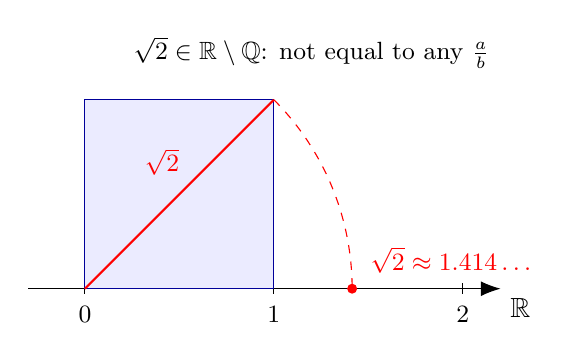
\begin{tikzpicture}[x=2.4cm, y=2.4cm]
	\draw[-{Latex[length=2.5mm]}] (-0.3,0) -- (2.2,0) node[below right] {$\mathbb{R}$};
	\foreach \x in {0,1,2} {\draw (\x,0.03) -- (\x,-0.03); \node[below=3pt, font=\small] at (\x,0) {$\x$};}
	\draw[blue!60!black, fill=blue!8] (0,0) rectangle (1,1);
	\draw[red, thick] (0,0) -- (1,1);
	\node[red, above left, font=\small] at (0.55,0.55) {$\sqrt2$};
	\draw[red, dashed] (0,0) ++(45:1.414) arc (45:0:1.414);
	\fill[red] (1.414,0) circle (1.8pt);
	\node[red, anchor=south west, font=\small] at (1.46,0.03) {$\sqrt2\approx1.414\ldots$};
	\node[font=\small, align=center] at (1.2,1.25) {$\sqrt2\in\mathbb{R}\setminus\mathbb{Q}$: not equal to any $\tfrac ab$};
\end{tikzpicture}
\end{document}
